\documentclass[a4paper,11pt]{article}
\usepackage{outlines}
\usepackage{graphicx}
\usepackage{url}
\usepackage{times}
\usepackage{natbib}
\usepackage{tabu}
\usepackage{graphicx}
\usepackage[nottoc]{tocbibind}
\usepackage{indentfirst}
\usepackage[margin=25mm]{geometry}
\title{Group 4 Report: Group Membership System}
\date{}
\author{
  Gaurav Pratap Chand\\
  \texttt{17318921}
  \and
  Shobhit Srivastava\\
  \texttt{17315016}
  \and
  Varun Bantwal Shenoy\\
  \texttt{17314890}
  \and
  Xu Zheng\\
  \texttt{17319652}
}
\begin{document}
\maketitle

\tableofcontents

\section{Requirements}
\subsection{Functional Requirement}
In this project, we need to build a group membership management service which allows a group of cooperating processes to work as a coherent group. Each of the group members should have a consistent view of the membership of that group. Besides, This service should be fault-tolerant and survive the failures of some of the members. The basic function concludes:
\begin{outline}
\1 Forming a group
\1 Node join a group and update membership for all the nodes
\1 Node leave a group and update membership for all the nodes
\1 A node can belong to multiple groups
\1 Provide an external client for interaction with these groups and nodes
\end{outline}
Each of these function should ensure that the nodes can have the updated membership. Besides, the failures need to be taken into consideration
\begin{outline}
\1 Node failure: if any node fails, it should be removed from the group
\1 Message loss
\1 Network Partition: We should ensure that there is only one leader that can respond to the external client in parted groups。
\end{outline}
Based on these requirements, we used Raft \cite{ongaro2014consensus} as the baseline algorithm, and the system design is implemented such a way that at any given time each node is one of three states, i.e. Leader, Follower and Candidate. In each group, there is only one leader at a time which is responsible for handling all request from external clients. The leader should sync updated membership to other servers and is responsible for sending heartbeat periodically to maintain the authority. The followers can respond to requests from leader and candidates, and it can become a candidate if it does not receive a valid heartbeat for a timeout period. Candidate performs election based on a term basis and can become a leader once it receives a majority(more than N/2) of votes. And we chose TCP as the network protocol to address the message loss problem.

\subsection{Non-functional Requirement}
We will analyse the non-functional requirement from several aspects:
\begin{outline}
\1 \textbf{Availability:} We should keep the service available during any membership change situation. As mentioned, we have a leader, and non-leader role is the group. We need to take care of the availability of any kinds of nodes failure. The leader can interact smoothly with an external client when a new node joins or existing node fails. Besides, if the leader node fails, we have to replicate it and select a new leader automatically within a short time.
\1 \textbf{Reliability:} In this project, the consistency of the membership is the key. We should ensure that every node has the same membership view no matter any of the nodes fails. Since it's not required to keep the time of the request logs from an external client, we only to make sure there is an eventual membership consistent for all the nodes and we do not need to keep the change history.
\1 \textbf{Scalbility:} We need to support multiple nodes and multiple groups, which means there should not be any limitation of the node number in one group and the system should have the ability to support multiple groups at the same time.
\end{outline}


\section{Specification}
There are five major functions in our system, including Group Forming, Node Joining, Node Failing, Network Partition Simulation, Query/List/Terminate Groups. Two executable files are responsible for these functions.
\subsection{Group Forming/Joining}
The first executable file named create\_servre.rb. It is responsible for Forming and Joining a Group. These two functions are supported by two very similar commands:
\begin{outline}
\1 ruby create\_server.rb nodeName groupName true (forming a group)
\1 ruby create\_server.rb nodeName groupName false (adding a node in an existing group)
\end{outline}
When forming a new group, This create\_server.rb executable file should be called with an initial Node as the default leader. In this case, the command needs four parameters, including node name, group name, the port number the node will run on, and a "true" to mark that this command is to create a new group with the given group name. Then the node will run on the port and start it role as the leader.
The second command is for adding a new node, which also needs four parameters. The only difference is that a "false" need to be provided to make sure it does not overwrite current groups with the same group name. If the group name does not exist, which means there is no such group for him to join, a new group with the provided name will be created automatically even a "false" has been provided, and the provided node will be the initial leader.
\subsection{External Client}
To support more operations, such killing node(simulate node failing and node leaving), network partition, membership query and terminate group, we created an external client that can send particular messages to the running nodes and external directory service. There are five different commands supported in this client.
\begin{center}
    \begin{tabular}{ | l | p{5cm} |} \hline
    1 & Kill One Node \\ \hline
    2 & Kill Multiple Nodes \\ \hline
    3 & Grep Membership from a Node \\ \hline
    4 & List of all the Groups \\ \hline
    5 & Terminate A Group \\ \hline
    \end{tabular}
\end{center}

\subsubsection{Node Leaving/Fail}
When there are multiple nodes running, we can call the API numbered as 1 to kill a node. It can kill the node provided by you no matter it is a leader or a follower. When a leader gets killed, the group will start a new round of the election. But if a follower gets killed, the leader will move this node after getting the commitment from all other nodes.
\subsubsection{Network Partition}
When you call the API numbered as 2, it will kill several nodes provided in the command. This command is used for simulating the network partition. After killing a group of nodes there are several situations, but we take care of these situations and make sure there is only one master in the devided groups. We will introduce how we simulate it and handle the different situations in section 4.
\subsubsection{Query Membership}
We call the API numbered as 3 in the client to query the membership of a node. After this API is called, the client will start a socket connection and send the message to that node to ask for membership. The membership is returned in a JSON format, including the leader information, all the follower's information and the group name.
\subsubsection{List Groups}
We call the API numbered as 4 in the client to ask for a group list from the external directory service. All the group information will be returned as JSON format, including all the nodes information, role information, and group name.
\subsubsection{Terminate Groups}
Terminate Group API(numbered as 5) is used to kill all the nodes in one group. When calling this API, the external client will first find all the information about this group and collection all the nodes port running in this group. Then the client will send terminate message to all these nodes.

\section{Architecture}
There are mainly three parts of our architecture. External Client, External Directory Service, and Node Group. You can check the figure 1 for the whole architecture overview. In this section, we will introduce these three modules and how they work with each other.

\begin{figure}
    \centering
    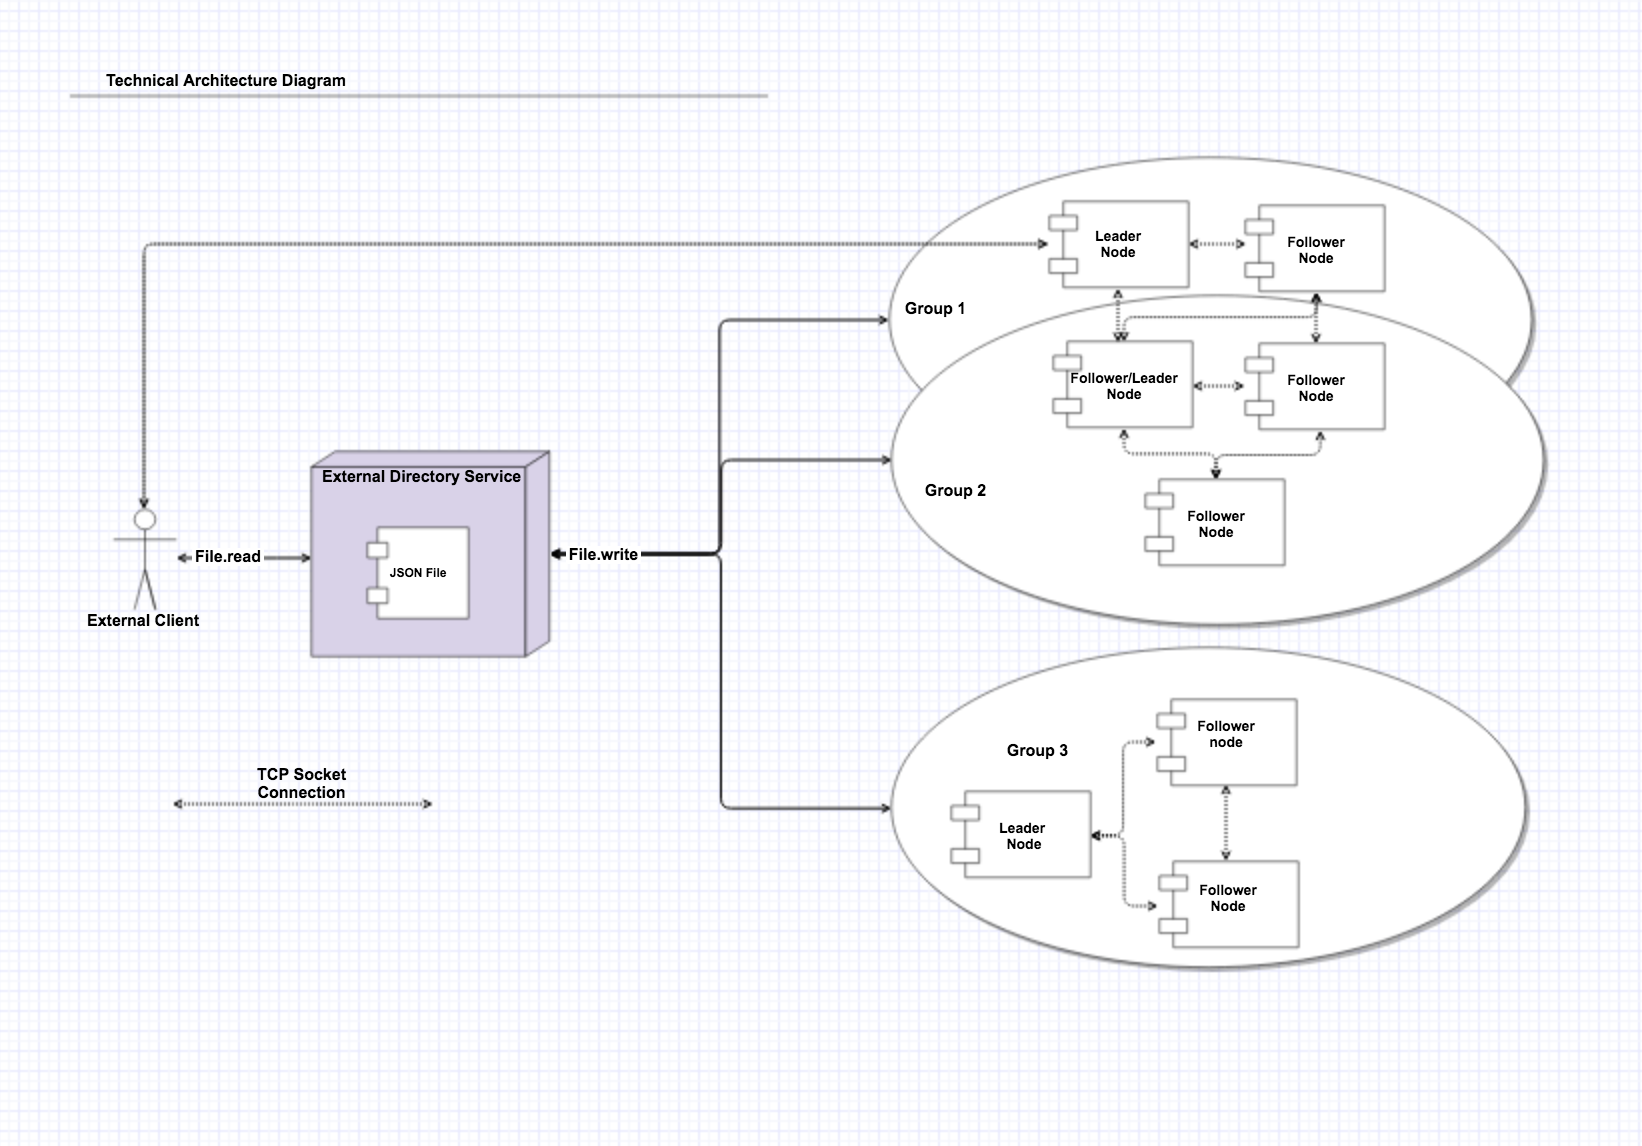
\includegraphics[scale=0.6]{assets/architectureDiagram}
    \caption{Architecture Diagram}
    \label{figure1: }
\end{figure}

\subsection{External Client}
External Client is built with programming language Ruby and TCP network protocol. It is used by a normal user to interact with the External Directory Service and Node Group. As mentioned in section two, five different methods are provided by this client. You can kill nodes, grep group information and terminate group with this client. It accesses External Directory Service by File.read() method provided by Ruby and cannot write the files. Besides, it uses TCP socket to interact with the nodes in the Node Group.
\subsection{External Directory Service}
External Client can find groups information through this external directory service. In our project, this "service" is a JSON file that can be accessed by both client and normal nodes. Each time the leader updates the membership, the information in this service should also be updated. The information includes the Group name, Node Name, Node Port and their roles in each group. Nodes access this service by the File.write() method provided by Ruby.
\subsection{Node Group}
Behind External Directory Service, there are multiple node groups. In each group, there are multiple nodes, and one node can belong to multiple groups. There are three different roles for the nodes. All nodes in the same group connect to each other with TCP socket.
\begin{outline}
\1 \textbf{Leader:} There is only one leader in each group at a time, and it is responsible for the membership updating. Besides, it sends heartbeat request regularly to all followers. The leader can become a follower if it gets a heartbeat message with higher term number.
\1 \textbf{Follower:} There can be many follower nodes in a group. They can only respond to requests from other servers. They can become candidates as long as it does not receive a valid heartbeat from a leader or candidate. But the followers cannot become leader directly
\1 \textbf{Candidate:} Candidate can perform election on a “Term” basis, and it can become a leader once it receives a majority of votes. If a candidate gets a vote request that has a larger term number, it will vote for that node and become a follower again and then update its term number.
\end{outline}
You can refer figure 2 to check more details of the relationship between them.
\begin{figure}
    \centering
    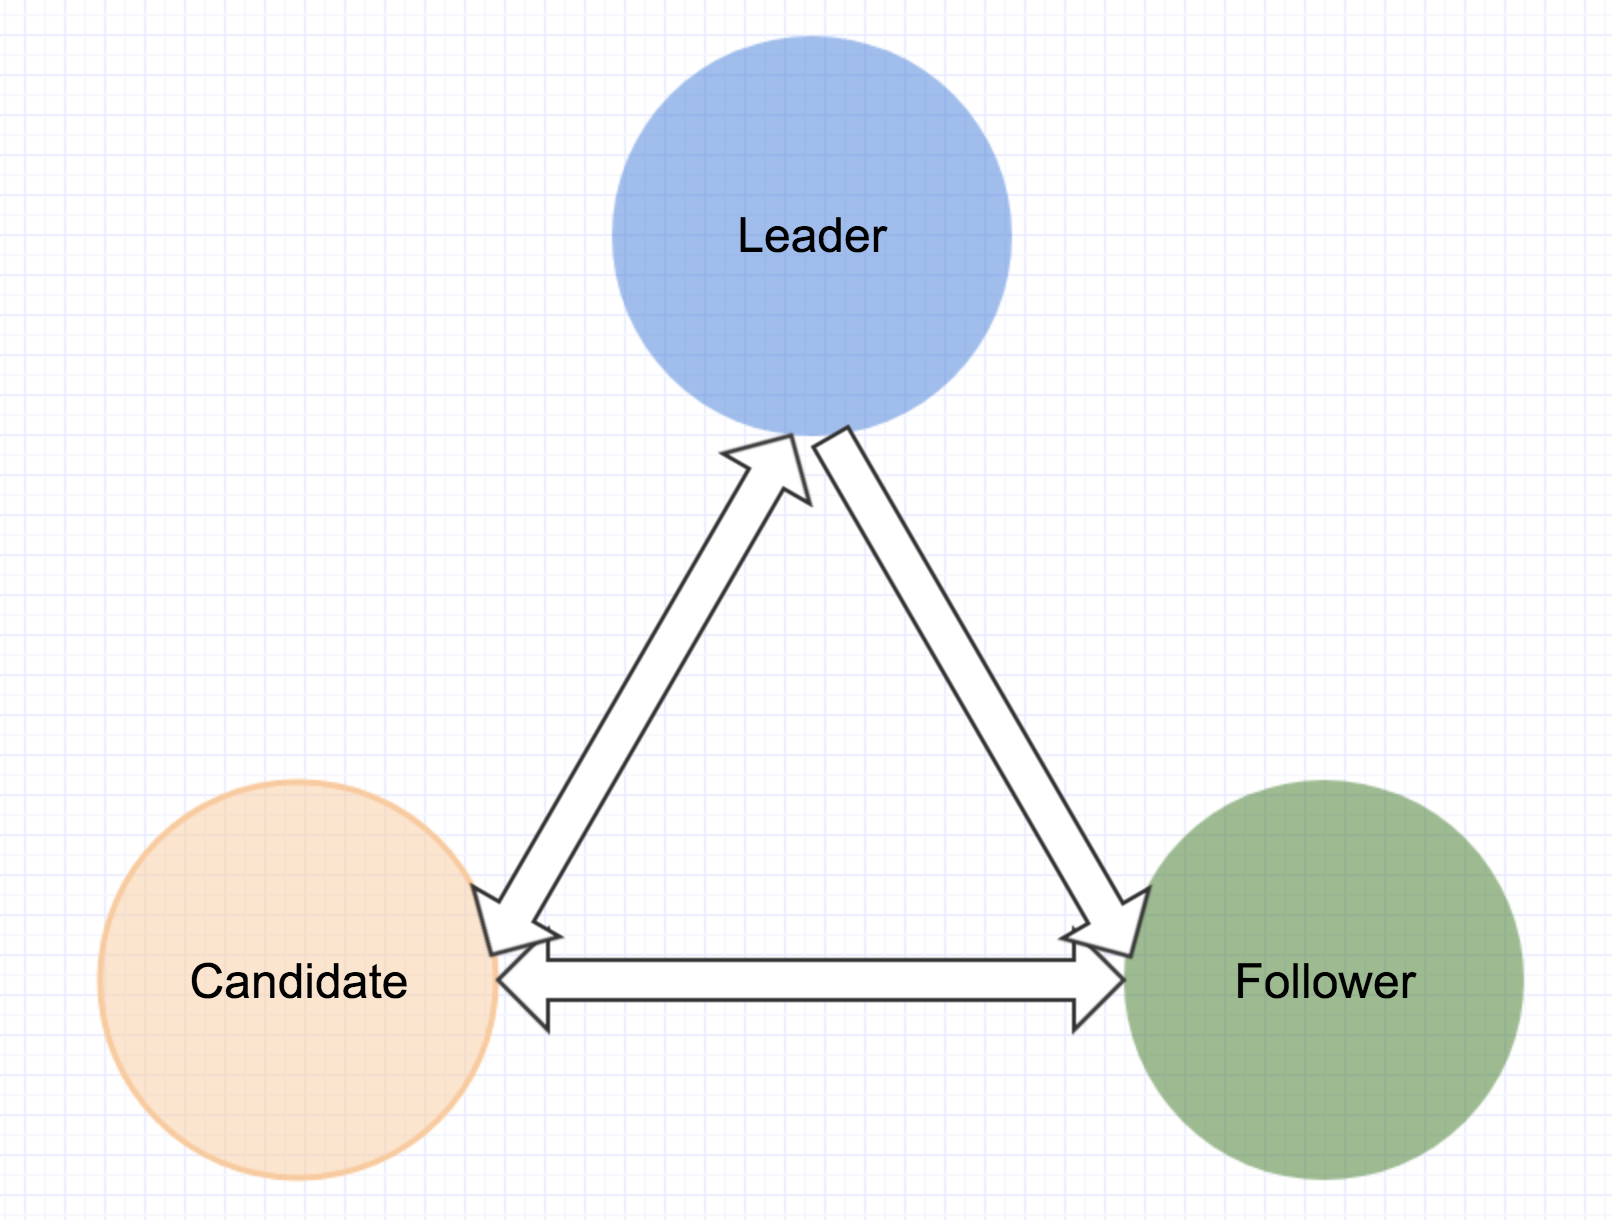
\includegraphics[scale=0.4]{assets/roleChange}
    \caption{Role Change}
    \label{figure2: }
\end{figure}

\section{Implementation}
\subsection{Basic Functions}
We will first introduce all the functions that will be used for dealing with different kinds of situations.
\begin{outline}
\1 \textbf{heartbeat:} The leader will call this function at the beginning of each timeout period. This function will send a heartbeat message to all the followers in that group, and followers need to respond this message to show that it's still alive.
\1 \textbf{log\_heartbeat\_reply:} Each time the leader gets an acknowledgement from the follower, it will add that follower in a repliers array. This array will be checked at the end of each heartbeat timeout period. At the meanwhile, the leader will also check the membership index carried in the acknowledgement if the index is smaller than current index. The leader will call return\_membership function to update the membership in that follower.
\1 \textbf{review\_last\_heartbeat\_round:} At the end of each timeout period, this function will be called. This function will check the count of acknowledgement from the followers. There is three situation:
  \2 It gets acknowledgement from all the nodes, then the leader will send heartbeat to all other nodes again and wait for another round of timeout.
  \2 It gets a majority of acknowledgement, then It will remove the fail nodes and then update the membership(will be introduced later on) and then send heartbeat to all left nodes again
  \2 It does not get the majority of acknowledgement. This case happens on network partition situation. In this case, the leader will become the candidate and start an election(will introduce this election function later).
  \2 Corner Case: If there are four nodes in one group and the network partition cased two groups, and each of them has two nodes, then the group with the original leader will keep a leader, and the nodes in another group will keep two candidates. We achieve this by giving the master node more weight. For example, the normal nodes weight one but the master weight 1.5. This can help us the fix the bugs in a balanced situation.
\1 \textbf{handle\_vote\_request:}. This function can be called by any roles when receiving a vote\_request. The node will check the term number; if the term number is bigger than its term number, a vote message will be sent to the owner of a vote request. Then the node updates its role to the follower.
\1 \textbf{return\_membership:} this function will be called in two cases:
  \2 When clients request membership, this function will be called and return the membership to the client.
  \2 When need to update the follower's membership as mentioned in log\_heartbeat\_reply function
\1 \textbf{update\_membership:} When a node gets return\_membership message, it will call this function. The membership index of that message will be checked firstly, then if the index is larger than current index, the membership and the index will be updated according to the data from the message.
\1 \textbf{confirm\_join\_request:} This function will be called when a new node wants to join this group. There is two situation for when calling this function:
  \2 If there is only one node(Leader itself): It will update its membership and send a committed message to the new node immediately.
  \2 There is more than one node: the leader will send confirm\_join\_request to all the followers and wait for a response.
\1 \textbf{check\_comitted:} Each time a leader get a commitment from the follower, it will call this method to check if it already got enough commitment(commit\_count>N/2). The leader will commit the join/leave request if it gets the majority of commitment. Otherwise, it will wait till next timeout. If it can not get enough commitment, the request can not be processed successfully.
\1 \textbf{launch\_candidacy} This function can be called by any roles. When this function gets called, the role of that node will become a candidate and launch a new term of election. There are 3 cases that can lead the nodes to call this function:
  \2 If the leader can not get a majority of acknowledgement.
  \2 If the follower cannot get heartbeat message within a timeout period.
  \2 If the candidate can not get enough votes.
\1 \textbf{acknowledge\_heartbeat:} This is the function used by nodes to respond the heartbeat message. When this function gets called, an acknowledgement message will be sent out, and the role of that node will become follower no matter what it is.
\1 \textbf{confirmed\_request:} This is function for follower nodes. Every time if a node wants to join or leave the group, the leader will send confirm\_join\_request. Followers respond the request with this function and send a commitment message to the leader.
\1 \textbf{handle\_vote}. When candidate nodes get a vote from other nodes, it will handle\_vote to log down the vote and check if it already gets the majority of votes. If the vote count is equal or bigger than NodesTotalNum/2 it will win the election and become the leader; then it starts sending a message to all the follower.
\end{outline}

\subsection{Node Join/Leave}
We will use a time sequence diagram to show the node join process: 

\begin{center}
    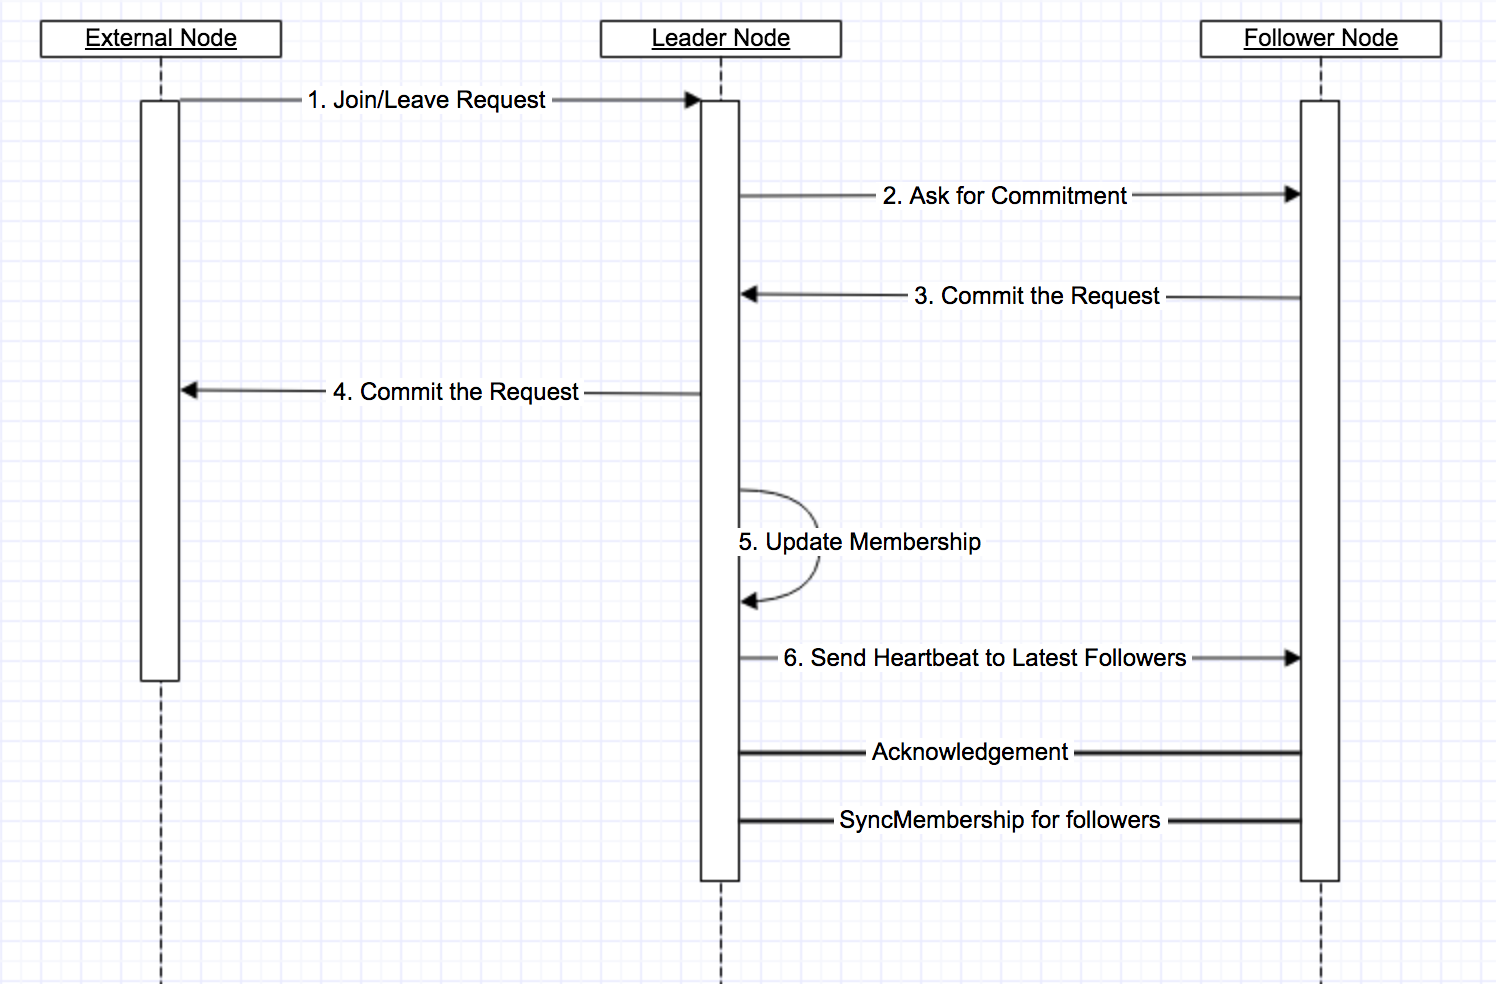
\includegraphics[scale=0.5]{assets/nodeJoin}
\end{center}

\begin{outline}
\1 External Node will first send a join request to leader Node
\1 After receiving the join request, leader Node needs to confirm the join request with all the followers
\1 Each follower who received the confirmation request will commit this request and send a response message to the leader.
\1 If leader get enough commitment, it will send a committed message to the external node and update the membership
\1 Then leader send heartbeat to the followers and sync the membership to the followers who have an old version of the membership
\end{outline}
\subsection{Leader Failure}
If the leader fails, the followers will wait for an election timeout period. The election timeout is a random time between 2-4 seconds to reduce the situation of vote split. The first node that reaches the timeout will become a candidate and start a new round of the election. If it gets more than N/2 votes, it will become the leader and start to send heartbeat and sync the membership for all other nodes. We will also use a time sequence diagram to show the process:
\begin{center}
    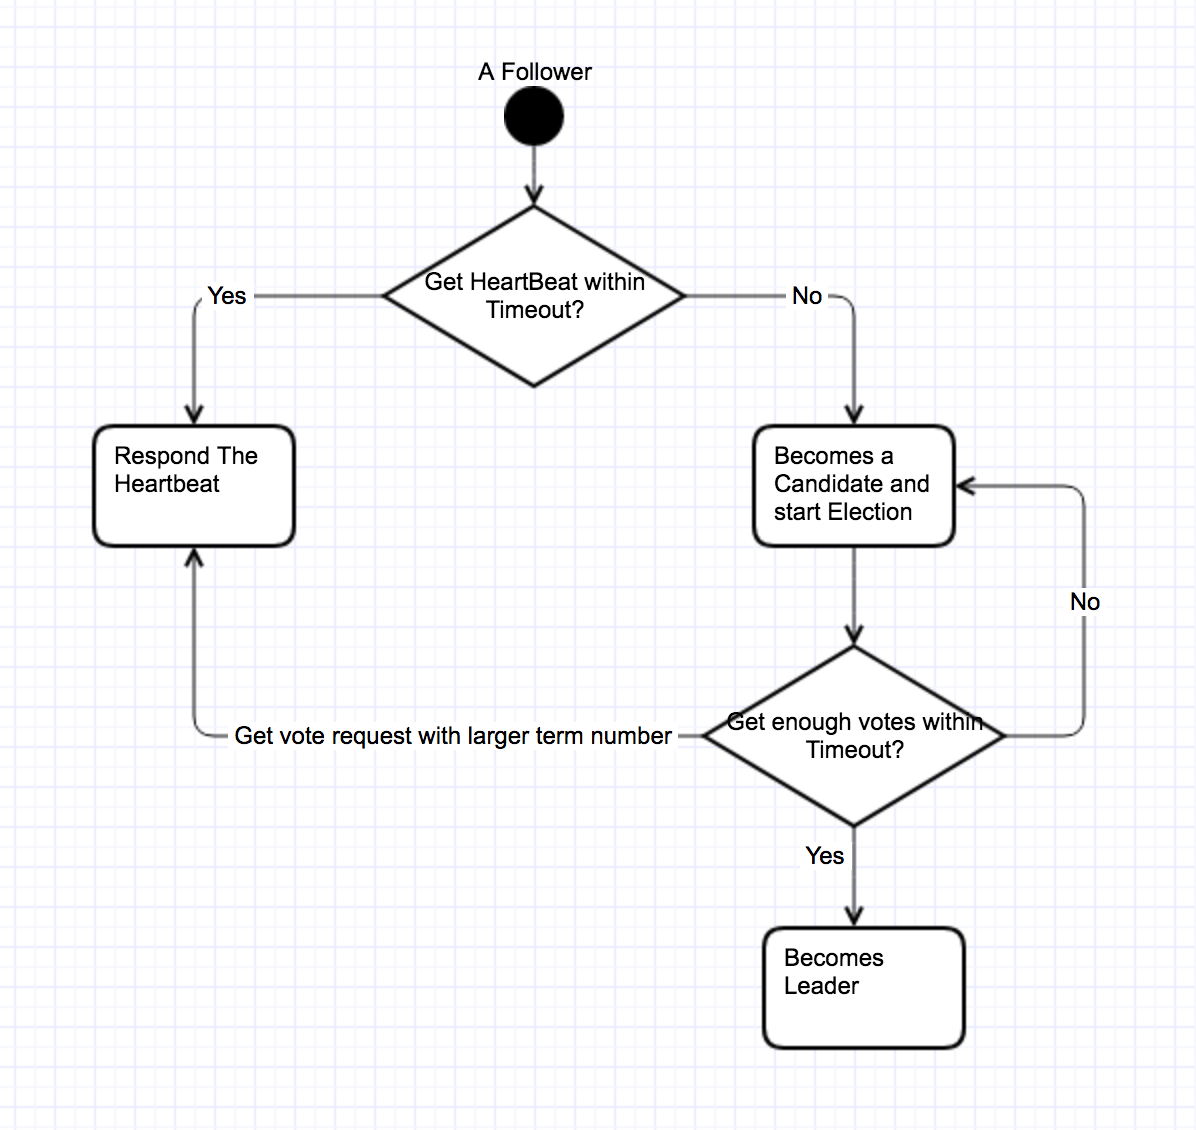
\includegraphics[scale=0.6]{assets/election}
\end{center}

\subsection{Network Partition}
When network partition happens, we keep there is only one leader in divided groups. There two situations of a network partition, balanced partition and unbalanced partition.
\begin{outline}
\1 \textbf{Unbalanced Partition:} For example, five nodes group is divided into a two nodes group and three nodes group. The group with more nodes will get a new leader since one of the nodes can still get a majority of votes or acknowledgement. The group with a smaller number of nodes will have no leader, and all the nodes become candidates and slaves again and again, but no one will win the election.
\1 \textbf{Balanced Partition:} For example, four nodes group is divided into two 2-nodes group. In this case, the group with the original leader will keep the leader, as we give the leader node more weight, 1.5, while all other nodes weight 1.
\end{outline}

\section{Testing}
In this section, we will describe some test cases and results of each test scenario. 
\subsection{Group Forming}
\begin{outline}
\1 Test Scenario: Create a new Group with an initial Leader Node
\1 Test Steps: 
  \2 Go to the project folder and run \emph{ruby create\_server.rb node1 group1 8008 true.}
  \2 Monitor the terminal and record the results. 
  \2 Start the external client \emph{ruby run.rb}, and grep membership from port number 8008
\1 Test Results
 \2 We can see that the node is running as the leader and trying to send heartbeat to all other nodes for each timeout period(even there are no followers).
 \2 When grepping the node, we can see the correct membership
\end{outline}

\subsection{Node Joining}
\begin{outline}
\1 Test Scenario: we already have a group after following the GroupForming test steps. We can then add a new node to this group.
\1 Test Steps:
  \2 Follow Group Forming steps to create a new group.
  \2 run \emph{ruby create\_server.rb node2 group1 8009} to create a news node in group1. The port number and node name should be different with the first one, but the group name should be the same.
  \2 Monitor the log from the terminal
  \2 Grep Latest Membership from the external client.
  \2 Add one more node. run \emph{ruby create\_server.rb node3 group1 8010}
  \2 Monitor the log from the terminal
  \2 Grep Latest Membership from the external client.
\1 Test Results
  \2 From the log we can observe that the node2 send join request to node1 and node1 committed this join request immediately
  \2 Node2 then send an acknowledgement to node1. Then node1 sync the membership to node2
  \2 Node1 send heartbeat to node2 and node2 response to this heartbeat by sending an acknowledgement message.
  \2 Grep Membership we can see there are two nodes in group1. Node1 is the leader, and node2 is the follower.
  \2 When adding one more node(node3), we can see node1 get join request and then send AskRequestCommit message to node2.
  \2 Node2 commit this request, then node1 committed this join request and updated its membership(including adding 1 to the index). Node3 get this commitment and send an acknowledgement to node1
  \2 Node1 sync membership to node3 then send heartbeat to node2 and node3
  \2 Grep membership with the external client we can see there are three nodes(node1 is the leader while node2 and node3 are the followers)
\end{outline}

\subsection{Follower Fail}
\begin{outline}
\1 Test Scenario: Simulate a node failure and test the group function well with correct membership for all the nodes.
\1 Test Steps
  \2 Follow the group forming and NodeJoining steps to create a group with one leader and two follower
  \2 Start the external client. And choose API 1: kill one node. Then input the node port 8010
  \2 Monitor the changes in the terminal and grep the latest membership
\1 Test Results
  \2 We can see the node3 process is terminated immediately. Wait for around 1 second, node1 detect the failure since the heartbeat cannot achieve node3 and got an error: Connection refused. Then node1 send remove commit request to left nodes(node2)
  \2 node2 commit this request and response to node1.
  \2 node1 marked this leave request as committed and update its membership and add 1 to the index. Then node1 sync this membership to node2 after it finds node2‘s membership index is smaller.
  \2 Grep the membership again, and you can find that there are only two nodes in the group1. One leader and one follower.
\end{outline}

\subsection{Leader Fail}
\begin{outline}
\1 Test Scenario: Simulate a Leader failure and test the group function well with a replicated leader and correct membership for all left nodes.
\1 Test Steps
  \2 Follow the group forming and NodeJoining steps to create a group with one leader and two follower
  \2 Start the external client. And choose API 1: kill one node. Then input the node port 8008(the port number of the leader nodes)
  \2 Monitor the changes in the terminal and grep the latest membership.
\1 Test Results
  \2 When we input the port number 8008, we can see the master is terminated immediately
  \2 Node2 and node3 stop send an acknowledgement. Wait for around 3 seconds, node2 becomes the candidate and send vote request to node1 and node3. But it gets an error when connecting to node1.
  \2 Node3 response the vote request and then node2 win the election.
  \2 Node2 become the new leader and then update the membership by removing the node1. Then it syncs the membership to node3 and starts sending heartbeat to node3.
  \2 When grepping the latest membership, you can see there are only two nodes. Node2 is the leader, and node3 is the follower.
\end{outline}

\subsection{Network Partition 1}
\begin{outline}
\1 Test Scenario: Simulate the network partition, i.e., the original group is divided into two different group. The first case is for the un-balanced group. A group with five nodes is divided into a group with two nodes and a group with three nodes.
\1 Test Steps
  \2 Follow the group forming and NodeJoining steps to create a group with one leader and four follower
  \2 Start the external client. And choose API 2: kill multiple nodes. Then input three node ports 8010 8011 8012
  \2 Monitor the changes in the terminal and grep the latest membership.
  \2 Again, follow the group forming and NodeJoining steps to create a group with one leader and four follower
  \2 Start the external client. And choose API 2: kill multiple nodes. Then input three node ports 8008 8009
  \2 Monitor the changes in the terminal and grep the latest membership.
\1 Test Results
  \2 When killing 8010 8011 8012, we can see the node1 and node2 becomes candidates and ask for the vote from other nodes continuously, but none of them can become a leader.
  \2 When killing 8008 8009, we observe that after waiting for around 3 seconds, nodes become a candidate and then win the election. Then node3 update the membership and sync the membership to all other nodes.
  \2 When grep membership again, we can see there are only three nodes in group1. node3 is the leader while node4 a node5 is the follower.
\end{outline}
\subsection{Network Partition 2}
\begin{outline}
\1 Test Scenario: The second network partition case is for balanced group division. A group with four nodes is divided into two group with the same nodes number. We make sure the group with the original leader keeps the leader, and there is no leader in another group.
\1 Test Steps
  \2 Follow the group forming and NodeJoining steps to create a group with one leader and three follower
  \2 Start the external client. And choose API 2: kill multiple nodes. Then input two node ports 8010 8011
  \2 Monitor the changes in the terminal and grep the latest membership.
  \2 Again, follow the group forming and NodeJoining steps to create a group with one leader and three follower
  \2 Start the external client. And choose API 2: kill multiple nodes. Then input three node ports 8008 8009
\1 Test Results
  \2 When killing 8010 8011, we can see the node1 find the partition and try to remove node3 and node4. After node2 commit this change request, node1 update the membership and sync the membership to node2.
  \2 When grep membership again, we can see there are only two nodes in group1. node1 is the leader while node2 is the follower.
  \2 When killing 8008 8009, we observe that node3 and node4 becomes a candidate and no node wins the election.
\end{outline}

\subsection{List all The Groups}
\begin{outline}
\1 Test Scenario: Query group information of all the groups.
\1 Test Steps: Start the external client and call the number 4 API
\1 Test Results: All the group information is listed in JSON format. We can also get leader info and follower info in each group.
\end{outline}

\subsection{Terminate a Group}
\begin{outline}
\1 Test Scenario: Terminate a group and terminate all the nodes in that group
\1 Test Steps
  \2 Follow the group forming and NodeJoining steps to create two groups.
  \2 Start the external client and list all the running groups.
  \2 Start the external client and call the number 5 API and provide the group name 
  \2 Monitor the changes in the terminal and grep the latest membership.
\1 Test Results
  \2 After running terminal group API you can see the nodes running in that group should be terminated
  \2 When grep membership again, we can see that the group number reduces by 1 and there is no information of the group provided by you
\end{outline}


\section{Individual contribution}
\begin{center}
    \begin{tabular}{ | l | l | p{5cm} |} \hline
    studentNumber & Name & Contribution\\ \hline
    17318921 & Gaurav Pratap Chand &Contributed in knowledge gathering and analysis of the technology to be used in the project. Made user interface in JSP in the initial stages. Slides Preparation. Worked on failure tolerance including network partitioning and node failure\\ \hline
    17315016 & Shobhit Srivastava & Studied multicast algorithm along with another group member for the project and taken knowledge transfer among the team. Implemented project through multicast in java to some extent later decided to go with ruby technology. Worked on failure tolerance including network partitioning and node failure. Support servral testing scenarios \\ \hline
    17319652 & Xu Zheng & Contributed to the implementation of key features of the project such as group forming, leaving and joining groups. Implementation of the election process and change the code to support multiple groups. Worked on making the slides and integrating all the documents to finalize the final report in Latex format \\ \hline
    17314890 & Varun Bantwal Shenoy & Studied raft algorithm for the project along with another group member and taken knowledge transfer to the team. Contributed to Failure tolerance including network partitioning and node failure. Documentation of the final report\\ \hline
    \end{tabular}
\end{center}

\section{Summary}
To realise this assignment, i.e., implementation of Group Membership Management for Distributed Systems, we were successfully able to design and implement a service which gives the members of the group a reliable perspective of its membership. The implementation takes care of failure usually emerges in any distributed system, i.e. message loss, processing or node failure, and network partitions. The consensus is achieved by Raft in the productive and practical way, i.e. by node leader election, where the chosen leader singularly makes decisions and transmission of membership. Only a little amount of mechanism is required by Raft to address the full consensus problem and also facilitate normal operation of the cluster during membership changes. Issues in client interaction with Raft, regarding the correctness, the issues of advancing read just queries and linearizability are particularly subtle. 
The implemented distributed system provides services such as, Group management, i.e. forming, joining, and leaving of group; monitoring of group members; responding to group member on demand; along with fault tolerance such as follower failing, leader failing, network partition, also Multiple groups support to cover the aspects of this task.
\bibliographystyle{chicago}
\bibliography{report}

\end{document}
